
\chapter{Plane Segmentation Development} \label{chap:plane-segmentation-development}

\section{RGB-D Approach}

In the previous century, it was almost unimaginable to parse the film in real time and interpret the frames.
Furthermore, the depth component seemed necessary to find plane segments in the pictures.
Since the RBG-Depth (RGB-D) sensors were only available in the form of expensive machines
like time-of-flight cameras or scanning 3-D laser range finders, \cite{articleFPSLinePrimitivesRGBD}
there were no possibilities for a broad usage of this technology, and thus, it saw little interest.
Nevertheless, there were several approaches for recognizing planar sections in the pictures.

\subsection{Rabbani Classification}

Rabbani \cite{articleSegPointCloudsSmoothnessConstraint} categorized contemporaneous plane segmentation algorithms
into three main categories:
\begin{enumerate}
\item \textbf{Edge-based segmentation}

This approach comprises two stages:

\begin{itemize}

\item Edge detection

It involves scanning the depth map for points in which there are some changes
in the local surface properties (like gradients or normals) above a designated threshold.

\item Point grouping

This part groups together points inside borders detected in the previous step.

\end{itemize}

One of the first successful applications of this method was done by Bhanu et al. \cite{Bhanu1986RANGEDP}
Another more recent work with promising results was published by Sappa et al. \cite{SappaEdgeDetectionStrategy}

\item \textbf{Surface-based segmentation}

Algorithms of this type try to merge points with similar local surface properties. Generally, there are two approaches:

\begin{itemize}

\item Bottom-up

It begins with selecting starting points and expanding from them using some predefined similarities.
It is worth noting that choosing these initial points is crucial as the results depend on them - i.e.,
you do not find segments without starting points within them.

\item Top-down

It starts by associating one big plane with all of the points in the picture.
Then, it cuts it into smaller pieces until it achieves a predefined fitting threshold.

\end{itemize}

One of the most prominent uses of this approach was published by Xiang et al. \cite{XiangSurfaceBasedSegmentation}.
They utilized the bottom-up approach, which generally is used much more often than the top-down technique.

\item \textbf{Scanline-based segmentation}

This approach treats rows or columns of pixels as scanlines.
It takes advantage of the fact that each scanline projection over a 3D surface creates a 3D line.
Ultimately, the technique consists of two stages:

\begin{itemize}

\item Line segments extraction

This stage involves processing scanlines to find line segments.

\item Line segments grouping

In this step, the extracted line segments are grouped with the neighbouring ones based on their similar surface properties
to form plane segments.

\end{itemize}

One of the first publications regarding this technique was made by Jiang et al. \cite{JiangOneOfTheFirstScanlineStrategies},
giving a groundbreaking performance at the time.
Natonek \cite{inproceedingsNatonekScanlinesForRobots} utilized a similar approach for robots just two years later, having promising results.

\end{enumerate}

These various techniques tackled plane segmentation from different perspectives.
However, most implementations required a large amount of computation,
thus rendering them inconvenient for real-time agent localization
due to the inability to process multiple frames per second.

\subsection{RGB-D Affordability}

Plane segmentation started drawing more attention at the beginning of the 2010s
when inexpensive RGB-D sensors (e.g. Microsoft Kinect) became available \cite{articleFPSLinePrimitivesRGBD}.
With the lower price came higher availability and more research.
Multiple algorithms were developed at that time.
They included different variations of plane extraction from the depth property with various optimisations,
among others:
\begin{itemize}
\item By Taguchi et al. \cite{inproceedingsEarlySLAMWithRANSACWithKinectSensor} - one that successfully uses
Simultaneous Location and Mapping (SLAM) with a Kinect 3D sensor.
It contains the Random Sample Consensus (RANSAC) \cite{articleRANSAC} - a widely used technique
in the Point Cloud Library (PCL) \cite{inproceedingsPCL};
\item By Salas-Moreno et al. \cite{inproceedingsPCAInSLAMToFindPlaneCandidates} - one that uses
Principal Component Analysis (PCA) to find plane candidates;
\item By Michael Kaes \cite{articleSLAMInfinitePlanes} - one that uses infinite planes and least-squares for mapping,
combined with minimal representation;
\item By Hsiao et al. \cite{inproceedingsKeyframeSLAM} - one that uses a keyframe-based approach
and is viable on Central Processing Unit (CPU)-only devices.
\end{itemize}
All of them utilize some variation of plane extraction from the depth property with a veraiety of optimizations.

\subsection{RGB-D To Point Cloud Mapping} \label{subsection:rgb-to-pc-mapping}

For every RGB-D algorithm, it is essential to correctly calculate the real point coordinates
based on the pixel location in the image.
The results map the factual world as seen by the camera.
The computation includes the focal length and the principal point (often the image centre)
and requires camera intrinsic parameters. 

In the first step, the camera matrix ($C$) is determined:
\begin{equation} \label{equation-camera-matrix}
	C = \begin{bmatrix}
		f_x &   0 & c_x & \\
		  0 & f_y & c_y & \\
		  0 &   0 &   1 & \\
	\end{bmatrix}
\end{equation}

where:
\begin{itemize}
\item $f_x$ is the focal length on x-axis
\item $f_y$ is the focal length on y-axis
\item $c_x$ is the principal point x-axis coordinate
\item $c_y$ is the principal point y-axis coordinate
\end{itemize}

Then, for each pixel with 2D coordinates $p(u,v)$
the world point $P(\mathbf{X},\mathbf{Y},\mathbf{Z})$ can be calculated as follows:
\begin{equation} \label{equation-world-point-calculation}
    \begin{cases}
        \mathbf{X} = \frac{( u - c_x ) \cdot \mathbf{Z}}{f_x} \\
        \mathbf{Y} = \frac{( u - c_x ) \cdot \mathbf{Z}}{f_x} \\
        \mathbf{Z} = d_p
    \end{cases}
\end{equation}

where:
\begin{itemize}
    \item $d$ is the depth component in RGB-D image for pixel $p(u,v)$
    \item $u$ is the pixel $p$ x-axis coordinate
    \item $v$ is the pixel $p$ y-axis coordinate
\end{itemize}

Figure~\ref{figure:Pinhole-Camera-Model} presents a visual explanation
of the pixel projection mapping described above.

\begin{figure}[H]
    \centering
    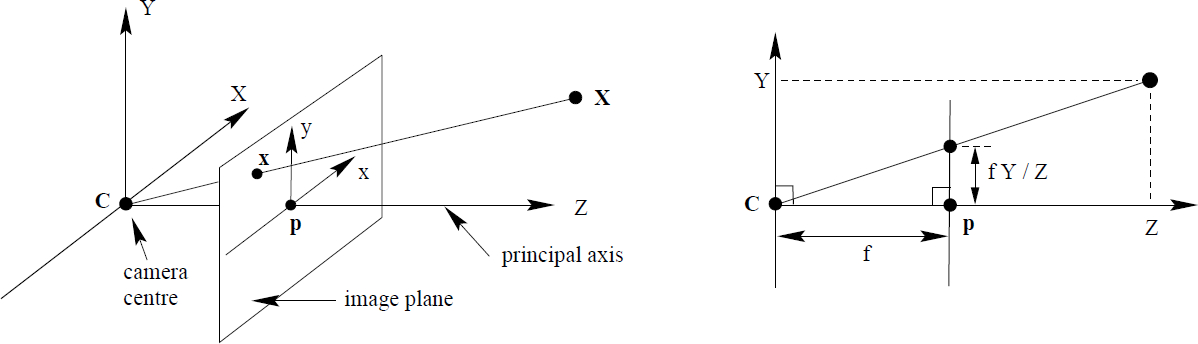
\includegraphics[width=1.0\textwidth]{images/psd/RGBD/Pinhole-Camera-Model.jpg}
    \caption{Pinhole Camera Model pixel projection. \cite{pinhole-camera-model}}
    \label{figure:Pinhole-Camera-Model}
\end{figure}

A set of 3D points, called Point Cloud, is obtained from the computation \cite{point-cloud}.
Points in the cloud are organized, therefore, adjacent points correspond to real neighbouring locations.
Consequently, the memory layout uses the same order, which speeds up the steps of many algorithms,
like searching for nearest neighbours.

\subsection{RGB-D State of the art}

One of the most successful algorithms developed using the RGB-D technique
is published by Zhang \cite{articleFPSLinePrimitivesRGBD} et al. discussed in more detail in the following chapter.
Their technique is based on scanlines.
The high-level overview of the algorithm can be seen in the Figure~\ref{figure:Flowchart-Zhang}.

\begin{figure}[H]
    \centering
    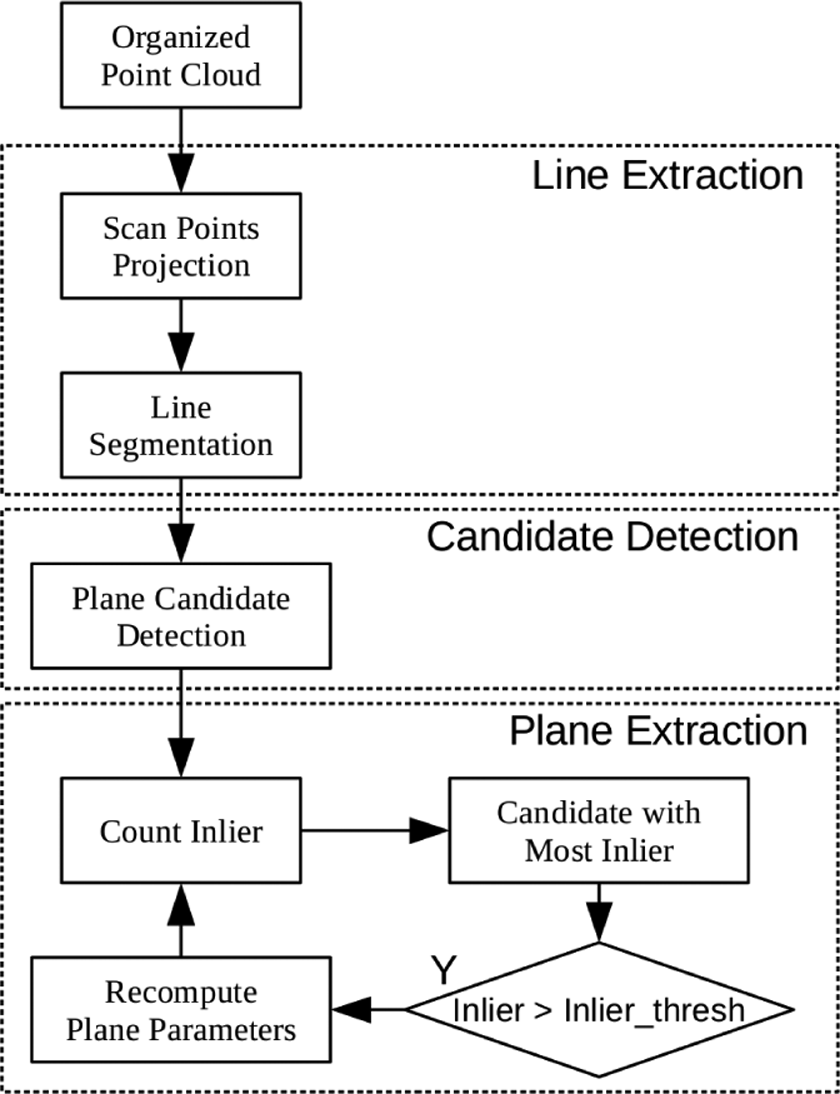
\includegraphics[width=0.6\textwidth]{images/psd/RGBD/Flowchart-Zhang.png}
    \caption{Flowchart of the plane segmentation approach. \cite{articleFPSLinePrimitivesRGBD}}
    \label{figure:Flowchart-Zhang}
\end{figure}

There are three main stages of the algorithm:

\begin{enumerate}

\item \textbf{Line Extraction}

The method, instead of looking for line segments on all possible scanlines,
selects a few scanlines periodically, e.g., every thirty rows.
It is worth mentioning that it is possible to select either rows or columns,
and we can adjust the interval size to achieve a compromise between accuracy and performance.

\begin{itemize}

    \item Scan Points Projection

    Each selected line is treated as a 2D laser scan for the purpose of segmentation.
    Then, for each pixel on these lines, the projection is calculated according
    to the equation~\ref{equation-world-point-calculation}
    from the RGB-D To Point Cloud Mapping section.~\ref{subsection:rgb-to-pc-mapping}

    \item Line Segmentation

    To extract line segments, the following algorithm is used:

    \begin{minipage}{\linewidth}
    \begin{algorithm}[H] \label{alg:line-regression}
        \SetAlgoLined
        
        Initialize sliding window size $N_f$. \\
        Fit a line to every $N_f$ consecutive points. \\
        Compute a line fidelity array. Each element of the array contains
        the sum of Mahalanobis distances between every three adjacent
        windows. \\
        Construct line segments by scanning the fidelity array for
        consecutive elements having values less than a threshold. \\
        Merge overlapped line segments and recompute line
        parameters for each segment.
        
        \caption{Line Regression \cite{articleFPSLinePrimitivesRGBD}}
    \end{algorithm}
    \end{minipage}

    This algorithm was initially proposed in a study by Arras and Siegwart. \cite{articleWithLineRegression}
    It yielded good results without much computational complexity.

\end{itemize}

\item \textbf{Plane Candidate Detection}

For each line segment, a plane candidate is calculated in the following way:

\begin{itemize}

\item Selection of points for local normals

The more points are selected, the more accurate the result, but with the cost of computational complexity.
The middle point for each line segment is a good compromise, which is confirmed empirically in the article.

\item Calculation of local normals

For each selected point, the smoothing region is chosen as a square with a fixed size (for example 20 pixels).
Then, for each region, the principal component analysis (PCA \cite{articlePCAInvention}) algorithm is executed,
which gives us the local normal.

\item Selection of plane candidates

Lastly, the valid points regarding PCA are chosen as an inlier (part of the plane) from the smoothing region.
Then, the local curvature is calculated,
and the inliers with the normals with curvature less than a maximum threshold are selected as plane candidates.

\end{itemize}

Example plane candidates result can be seen in the Figure~\ref{figure:Scanlines-and-plane-candidates-visualization}

\begin{figure}[H]
    \centering
    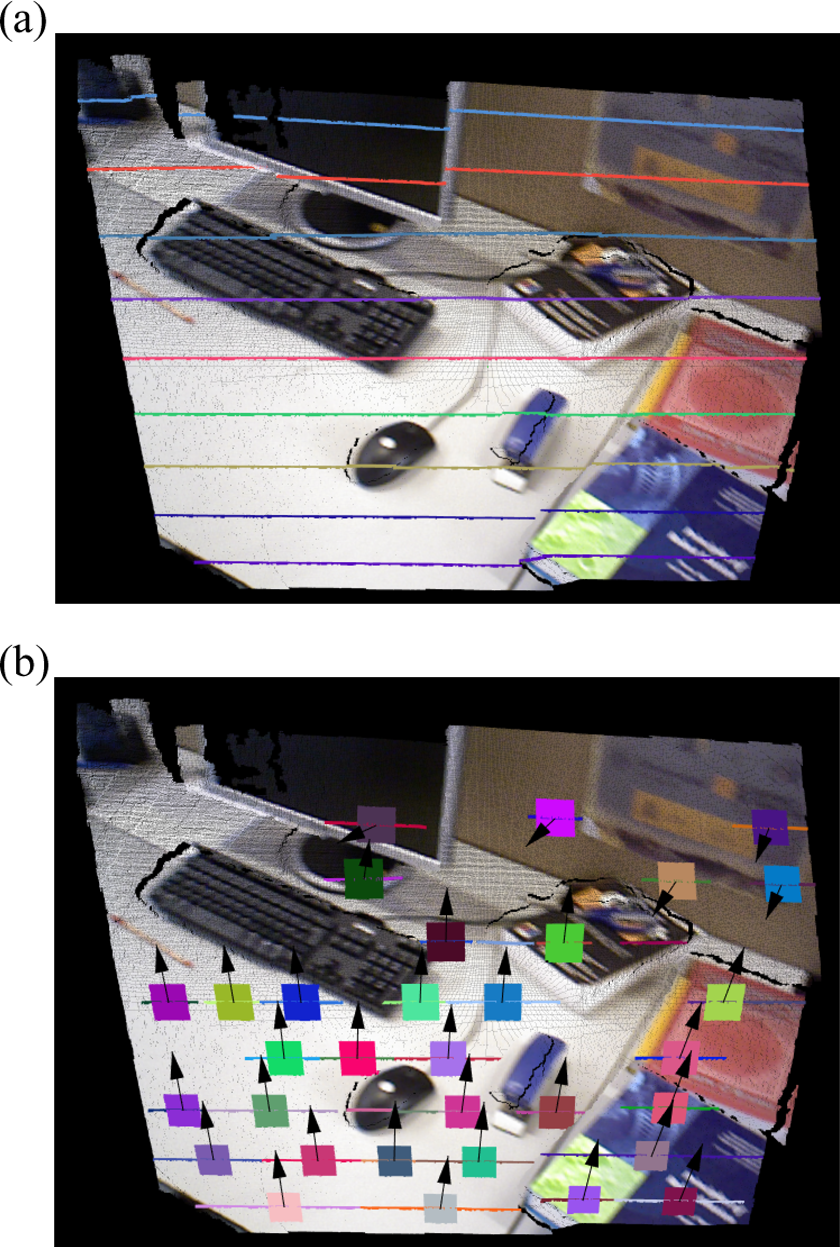
\includegraphics[width=0.6\textwidth]{images/psd/RGBD/scanlines-and-plane-candidates-visualization.png}
    \caption{Examle showing plane candidates calculation. \cite{articleFPSLinePrimitivesRGBD}
    (a) Colored lines are scanlines
    (b) Each plane candidate is represented by part of the line segment (colored line),
    normal smoothing region (colored square) and local normal emerging from the middle point (black arrow)}
    \label{figure:Scanlines-and-plane-candidates-visualization}
\end{figure}

\item \textbf{Plane Extraction}

For plane extraction, the recursive algorithm is used, which is presented in the Algorithm~\ref{alg:recursive-plane-extraction}
It takes every plane candidate and discards each with its inlier $N_s$ smaller than the minimal threshold $N_{s thresh}$.
Then, it calculates the quality of the inlier by counting how many neighbours within range $d_n$
are closer to the plane than a distance threshold $d_{\tau}$.
The candidate is also invalidated if the number of valid points is smaller than the minimal threshold $N_{\xi_{thresh}}$.
Next, the biggest approved inlier $N_{\xi_{max}}$ is considered to be part of the plane segment from the final result.
Ultimately, principal component analysis \cite{articlePCAInvention} is calculated again for the selected candidate $N_{\xi_{max}}$,
and the actual inlier of the chosen plane segment is deducted directly from the point cloud.
After adding the plane segment to the result set,
the plane candidate $N_{\xi_{max}}$ is removed from the possibilities for the next iterations.
This sequence of actions is repeated recursively until there are no valid plane candidates.

    \begin{minipage}{\linewidth}
    \begin{algorithm}[H] \label{alg:recursive-plane-extraction}
        \SetAlgoLined
        \KwIn{plane candidates $\hat{\xi_i},i=1,2,\cdots,n$.}
        \KwOut{plane segments $\xi_j,j=1,2,\cdots,m$.}
        \While{number of valid plane candidates $\neq 0$}{
            initialize maximum inlier number $N_{\hat{\xi_{max}}} \leftarrow 0$,
            corresponding plane parameters $\hat{\xi_{max}} \leftarrow invalid$. \\
            \For{$i = 1$ \textbf{to} $n$}{
                \If{$\hat{\xi_i}$ is invalid}{
                    count number of valid points $N_s$ in normal smoothing region \\
                    \eIf{$N_s > N_{s thresh}$}{
                        count number of valid points $N_{\hat{\xi_i}}$ by point-plane
                        distance threshold $d_{\tau}$ and neighbour distance
                        threshold $d_n$ \\
                        \If{$N_{\hat{\xi_i}} > N_{\hat{\xi_{max}}}$ \textbf{and} $N_{\hat{\xi_i}} > N_{\hat{\xi_{thresh}}}$}{
                            $N_{\hat{\xi_{max}}} = N_{\hat{\xi_i}}$
                        }
                    }{
                        $\hat{\xi_i} \leftarrow invalid$
                    }
                }
            }
            \eIf{$N_{\xi_{max}} > N_{\xi_{thresh}}$}{
                recompute plane parameter $\hat{\xi_{max}}$ using all the inlier \\
                save result plane $\xi_j \leftarrow \hat{\xi_{max}}$ \\
                delete inlier in point cloud data
            }{
                \textbf{break}
            }
        }
        \caption{Recursive plane extraction \cite{articleFPSLinePrimitivesRGBD}}
    \end{algorithm}
    \end{minipage}

\end{enumerate}

\section{RGB Approach} \label{sec:rgb-approach}

With the recent boom in artificial intelligence,
especially in neural networks, the scientific community has realized,
that it is possible to get rid of all depth scanners
and extract information about plane segments from simple RGB images, similar to our brain.
The first successful attempt using a neural network to detect plane segments from a plain RGB was
PlaneNet brought by Liu et al. \cite{articlePlaneNet}
It took advantage of the recent advancement
in neural network technology - Dilated Residual Network (DRM) \cite{inproceedingsDetailedResidualNetworks},
which was published just a year prior.
This success drew much attention to the topic, and since then, there have been multiple enhancements and progressions.
Based on the PlaneNet, SlamCraft was introduced by Rambach et al. \cite{inproceedingsSlamCraft} - a SLAM framework,
which proved, that monocular SLAM systems are feasible with adequate neural network untilization.
Yu et al. \cite{inproceedingsEncoderDecoderApproach} tackled the problem from a different perspective.
They have proposed a two-stage algorithm using an encoder-decoder approach and achieved promising results.
A big step forward was the introduction of PlaneRCNN by Liu et al. \cite{articlePlaneRCNN}
They used mask R-CNN \cite{inproceedingsMaskRCNN} - a recent innovation in a neural network to computer vision.
The state-of-the-art advancements are brought by Yaxu Xie et al. in the form of PlaneSegNet \cite{inproceedingsPlaneSegNet}.
This framework achieves great results and was proved SLAM-worthy by
Shy et al. in the form of Structure PLP-SLAM \cite{inproceedingsPLPSLAM}, which uses PlaneSegNet for plane segmentation.

\subsection{Begin: Ask if needed neural network theory}

\par

All of the methods addressed in Section~\ref{sec:rgb-approach} use some variation of neural networks.
Why is that the case?
Well, many years ago, Kurt Hornik, Maxwell Stinchcombe, and Halbert White proved mathematically that multilayered feedforward neural networks are universal approximators. \cite{HORNIK1989359}
So why haven't they been widely spread and entangled in multiple tasks?
Training a neural network is highly resource-intensive.
To train a neural network, huge amounts of data and computation are required, and thus, the hardware capabilities prevented the scientific community from satisfactory results.
With the era of GPUs, the situation has changed and we can see the presence of neural networks almost everywhere.
In the section~\ref{subsec:neural-networks} the basic principles of neural networks are presented.

\subsection{Neural Networks} \label{subsec:neural-networks}

\subsection{End: Ask if needed neural network theory}

\subsection{RGB state-of-the-art - PlaneSegNet}

The current state-of-the-art RGB plane segmentation is represented by PlaneSegNet
proposed by Yaxu Xie et al. \cite{inproceedingsPlaneSegNet}
The architecture is based on the YOLACT++ instance segmentation framework published by
Bolya et al. \cite{articleYOLACT} with added optimizations in some of the modules.
The general overview of the framework can be seen in Figure~\ref{figure:PlaneSegNet-Architecture}.
The architecture is quite complex and consists of:

\begin{itemize}

\item Encoder

Produces a group of multi-scale feature maps ${P_3, P_4, P_5, P_6, P_7}$.

\begin{itemize}

\item Backbone Network
It is a deep residual network based on the ResNet by He et al. \cite{inproceedingsResNet}
\item Feature Pyramid
Feature Pyramid Network structure based on the work of Lin et al. \cite{inproceedingsFPN}

\end{itemize}

\item Residual Feature Augmentation

Apart from the standard connection, layer $C_5$ of the backbone is connected to the prediction layer $P_5$
through the Residual Feature Augmentation brought by Guo et al. \cite{inproceedingsResidualFeatureAugmentation}
It improves the context of the spatial placement of the features.

\item Prediction Head
For each layer of the Feature Pyramid Network, it produces $c$ class confidences,
four bounding box regressors, and $k$ mask coefficients.

\item Fast Feature NMS

The most significant innovation brought by PlaneSegNet.
It aims to enhance overlapping instances detection reliability.
It is discussed more in detail in the Subsection~\ref{subsubsec:fast-feature-nms}.

\item ProtoNet

It is a convolutional neural network.
It takes the feature maps from the $P_3$ layer and predicts $k$ channels for prototype masks.

\item Mask Assembly

It assembles prototype masks based on the following linear combination equation:

\begin{equation} \label{eq:mask-assembly}
    M = \sigma(P\mathbf{C_T})
\end{equation}

where:
\begin{itemize}
    \item $\sigma$ is a non-linear sigmoid function
    \item $P$ is a tensor of dimensions $h \times w \times k$ containing prototype masks
    \item $\mathbf{C}$ is a matrix of dimensions $n \times k$ containing mask coefficients
    for the output of Fast Feature NMS~\ref{subsubsec:fast-feature-nms}
\end{itemize}

\end{itemize}

\begin{figure}[H]
    \centering
    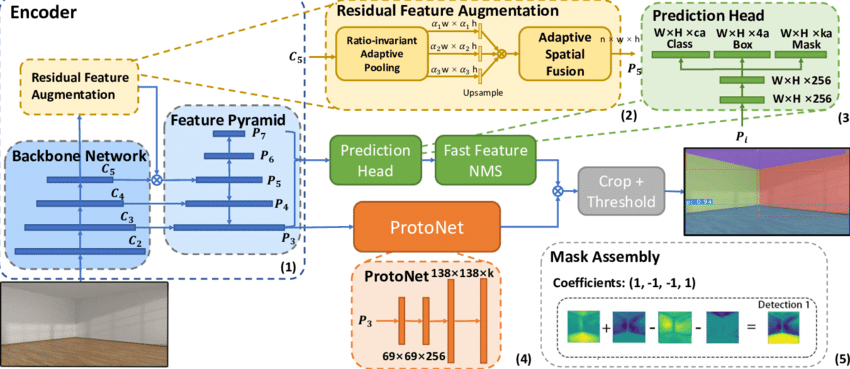
\includegraphics[width=1.0\textwidth]{images/psd/RGB/PlaneSegNetArchitecture.png}
    \caption{PlaneSegNet Architecture. (1) Encoder (2) Residual Feature Augumentation
    (3) Prediction Head (4) ProtoNet (5) Mask Assembly \cite{inproceedingsPlaneSegNet}}
    \label{figure:PlaneSegNet-Architecture}
\end{figure}

\subsubsection{The loss function}

It takes into consideration each of the mask, confidence, and bounding box (localization) losses.
It is represented with the following equation:

\begin{equation} \label{eq:loss-function}
    \mathscr{L}(x,C,B,M) = \frac{1}{N}(\mathscr{L}_{conf}(x,C)
    + \alpha\mathscr{L}_{loc}(x,B,B_{gt})
    + \beta\mathscr{L}_{mask}(x,M,M_{gt}))
\end{equation}

where:
\begin{itemize}
    \item $C$ is a confidence representation
    \item $B$ is a bounding box (localization) representation
    \item $M$ is a mask representation
    \item $N$ is the number of positive matchings
    \item $\mathscr{L}_{conf}$ and $\mathscr{L}_{loc}$ are loss function taken from the single-shot detector
    presented by Liu et al. \cite{inproceedingsSingleShotDetector}
    \item $\mathscr{L}_{mask}$ is the pixel-wise binary cross entropy between the ground truth and predicted masks.
\end{itemize}

\subsubsection{Fast Feature Non-maximum Suppression} \label{subsubsec:fast-feature-nms}

It was observed, that strongly overlapping bounding boxes often don't belong to the same object.
Because of that, usage of the classic NMS method brings unnecessary calculation overhead.
To resolve this issue, a new method is introduced, Fast Feature Non-maximum Suppression.
The technique is based on the research of Salcheider and Niels,
who came up with Feature Non-maximum Suppression. \cite{inproceedingsFeatureNMS}

\par

This method is presented in the form of Algorithm~\ref{alg:fast-feature-nms}
The $N_1$ and $N_2$ are thresholds for the common area of overlapping bounding boxes ($IoU$).
If $IoU$ is smaller than $N_1$, the boxes are considered to be from different objects.
However, if $IoU$ is bigger than $N_2$, the boxes are considered to be from the same object.
Finally, if $IoU$ is between $N_1$ and $N_2$, the similarity $S_i$ of the objects is calculated,
and if it is below the given likeness threshold $T$, the boxes are considered to be from different objects.
It is worth noting that this approach adds minimal overhead compared to the Fast NMS.

\begin{minipage}{\linewidth}
\begin{algorithm}[H] \label{alg:fast-feature-nms}
    \SetAlgoLined
    \KwIn{$P \leftarrow Sort(Proposals)$ with Scores, $D \leftarrow \emptyset$ }
    $X^{triu} \leftarrow GetPairwiseIoU(P)$ \\
    $K \leftarrow max(X^{triu})$ column-wise \\
    \eIf{$K_i \leq N_1$}{
        $PUSH(p_i,D)$
    }{
        \If{$K_i \leq N_2$}{
            $C^{triu} \leftarrow GetCosineSim(p,D)$ \\
            $S \leftarrow max(C^{triu})$ column-wise \\
            \If{$S_i \leq T$}{
                $PUSH(p_i,D)$
            }
        }
    }
    \textbf{return} $D$
    \caption{Fast Feature NMS \cite{inproceedingsPlaneSegNet}}
\end{algorithm}
\end{minipage}
